\documentclass[tikz,border=5mm]{standalone}
\usepackage{pgfplots}
\usepackage{amsmath}
\pgfplotsset{compat=1.18}

% Explicit RGB color definitions
\definecolor{edgeblue}{RGB}{0, 0, 128}
\definecolor{fillcyan}{RGB}{214, 239, 250}
\definecolor{dotred}{RGB}{204, 24, 66}

\begin{document}
	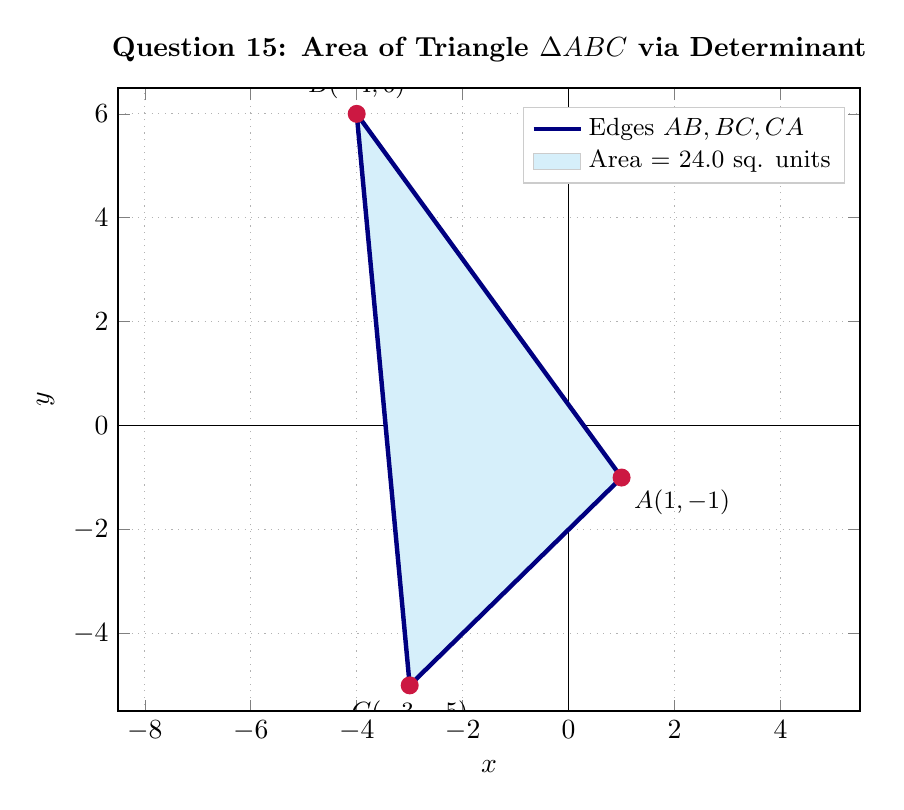
\begin{tikzpicture}
		\begin{axis}[
			width=11cm, height=9.5cm,
			title={\textbf{Question 15: Area of Triangle $\Delta ABC$ via Determinant}},
			xlabel={$x$}, ylabel={$y$},
			xmin=-8.5, xmax=5.5,
			ymin=-5.5, ymax=6.5,
			xtick={-8,-6,-4,-2,0,2,4},
			ytick={-4,-2,0,2,4,6},
			grid=both,
			grid style={dotted, gray!60},
			axis line style={black, thick},
			legend cell align={left},
			legend style={at={(0.98,0.97)}, anchor=north east, font=\small, draw=gray!40}
			]
			% Origin axis lines
			\draw[black, thin] (axis cs:0,-5.5) -- (axis cs:0,6.5);
			\draw[black, thin] (axis cs:-8.5,0) -- (axis cs:5.5,0);
			
			% Triangle fill and edges
			\addplot[line width=1.6pt, draw=edgeblue, fill=fillcyan] coordinates {(-4,6) (-3,-5) (1,-1) (-4,6)};
			\addlegendentry{Edges $AB, BC, CA$}
			
			% Area legend entry
			\addlegendimage{area legend, fill=fillcyan, draw=none}
			\addlegendentry{Area = 24.0 sq. units}
			
			% Vertices and labels
			\node[circle, fill=dotred, inner sep=2.3pt] at (axis cs:-4,6) {};
			\node[above=2pt, font=\small] at (axis cs:-4,6) {$B(-4, 6)$};
			
			\node[circle, fill=dotred, inner sep=2.3pt] at (axis cs:-3,-5) {};
			\node[below=2pt, font=\small] at (axis cs:-3,-5) {$C(-3, -5)$};
			
			\node[circle, fill=dotred, inner sep=2.3pt] at (axis cs:1,-1) {};
			\node[below right=1pt, font=\small] at (axis cs:1,-1) {$A(1, -1)$};
		\end{axis}
	\end{tikzpicture}
\end{document}